\documentclass[a4paper]{article}

\usepackage{fullpage} % Package to use full page
\usepackage{parskip} % Package to tweak paragraph skipping
\usepackage{tikz} % Package for drawing
\usepackage{amsmath}
\usepackage{hyperref}
\usepackage{ctex}
\usepackage{amssymb}
\usepackage{amsthm}

\renewcommand\thefigure{\thesection.\arabic{figure}}
\makeatletter
\@addtoreset{figure}{section}
\makeatother

\makeatletter
\renewcommand \theequation {%
	\ifnum \c@section>\z@ \@arabic\c@section.\fi \ifnum \c@subsection>\z@
	\@arabic\c@subsection.\fi\ifnum \c@subsubsection>\z@
	\@arabic\c@subsubsection.\fi\@arabic\c@equation}
\@addtoreset{equation}{section}
\@addtoreset{equation}{subsection}
%\setcounter{section}{-1}
\makeatother

\title{最优化方法作业9}
\author{罗雁天 \\
2018310742}
\date{\today}

\begin{document}

%\maketitle
\newcommand{\HRule}{\rule{\linewidth}{0.5mm}}
\begin{titlepage}
	\begin{center}
		% Upper part of the page
		
\includegraphics[width=0.4\textwidth]{Tsinghua2.png}\\[1cm]
		\textsc{\Large \texttt{清华大学电子工程系}}\\[1cm]
		% Title
		\HRule \\[1cm]
		{\Huge \bfseries 最优化方法作业9}\\[0.4cm]
		\HRule \\[3.5cm]
		% Author and supervisor
		\begin{minipage}{0.4\textwidth}
			\begin{center}
				\Large
				\begin{tabular}{cc}
					\texttt{作者:} & 罗雁天 \\[0.5cm]
					\texttt{学号:} & 2018310742 \\[0.5cm]
					\texttt{日期:} & \today
				\end{tabular}
			\end{center}
		\end{minipage}
		\vfill
	\end{center}
\end{titlepage}

\section{}
考虑如下非线性规划问题:
\begin{equation}
\begin{aligned}
\min\quad&x_2 \\
s.t.\quad&-x_1^2-(x_2-4)^2+16\ge 0\\
&(x_1-2)^2+(x_2-3)^2-13=0
\end{aligned}
\end{equation}
判断下列各点是否为最优解:
$x^{(1)}=[0,0]^T,x^{(2)}=\left[\frac{16}{5}, \frac{32}{5}\right]^T,x{(3)}=\left[2,3+\sqrt{13}\right]^T$

\begin{proof}[解]
	计算导数及Lagrange函数如下:
	\begin{equation}
	\begin{aligned}
	\bigtriangledown f(x)&=[0,1]^T \\
	\bigtriangledown g(x)&=[-2x_1,-2(x_2-4)]^T \\
	\bigtriangledown h(x)&=[2(x_1-2),2(x_2-3)]^T \\
	L(x,w,v)&=f(x)-wg(x)-vh(x) \\
	\bigtriangledown_x L&=\bigtriangledown f(x)-w\bigtriangledown g(x)-v\bigtriangledown h(x) \\
	&=\left[
	\begin{array}{c}
	2wx_1-2vx_1+4v \\
	2wx_2-2vx_2+1-8w+6v
	\end{array}
	\right]\\
	\bigtriangledown_x^2 L&= \left[
	\begin{array}{cc}
	2w-2v & 0\\
	0 & 2w-2v
	\end{array}
	\right]
	\end{aligned}
	\end{equation}
	对于$x^{(1)}$,是可行解,且$g(x),h(x)$均为紧约束,则KKT条件为:
	\begin{equation}
	\left\{
	\begin{array}{c}
	4v=0 \\
	1-8w+6v=0 \\
	w\ge 0
	\end{array}
	\right.
	\end{equation}
	解得$w=\frac{1}{8},v=0$满足一阶必要条件,因此$x^{(1)}$是KKT点。
	解方程组:
	\begin{equation}
	\left\{
	\begin{array}{c}
	\bigtriangledown g(x^{(1)})^Td=0 \\
	\bigtriangledown h(x^{(1)})^Td=0
	\end{array}
	\right.
	\end{equation}
	得到$d=0$,因此方向集$G=\{d|d\neq0,\bigtriangledown g(x^{(1)})^Td=0,\bigtriangledown h(x^{(1)})^Td=0\}=\emptyset$,因此$\bigtriangledown_x^2 L$在$G$上可以看做是半正定的,所以$x^{(1)}$是局部最优解
	
	对于$x^{(2)}$,是可行解,且$g(x),h(x)$均为紧约束,则KKT条件为:
	\begin{equation}
	\left\{
	\begin{array}{c}
	\frac{32}{5}w-\frac{12}{v}=0 \\
	1+\frac{24}{5}w-\frac{34}{5}v=0 \\
	w\ge 0
	\end{array}
	\right.
	\end{equation}
	解得$w=\frac{3}{40},v=\frac{1}{5}$满足一阶必要条件,因此$x^{(2)}$是KKT点。
	解方程组:
	\begin{equation}
	\left\{
	\begin{array}{c}
	\bigtriangledown g(x^{(2)})^Td=0 \\
	\bigtriangledown h(x^{(2)})^Td=0
	\end{array}
	\right.
	\end{equation}
	得到$d=0$,因此方向集$G=\{d|d\neq0,\bigtriangledown g(x^{(1)})^Td=0,\bigtriangledown h(x^{(1)})^Td=0\}=\emptyset$,因此$\bigtriangledown_x^2 L$在$G$上可以看做是半正定的,所以$x^{(2)}$是局部最优解
	
	对于$x^{(3)}$,满足约束条件,$g(x)$是不起作用约束,$h(x)$是起作用约束,则KKT条件为:
	\begin{equation}
	\left\{
	\begin{array}{c}
	w=0 \\
	1-2\sqrt{13}v=0 \\
	\end{array}
	\right.
	\end{equation}
	解得$w=0,v=\frac{\sqrt{13}}{26}$.
	求方向集$G$:
	\begin{equation}
	\bigtriangledown h(x^{(2)})^Td=0
	\end{equation}
	得$G=\{d|d=[d_1,0]^T,d_1\neq0\}$,计算$\bigtriangledown_x^2 L(x,0,\frac{\sqrt{13}}{26})$如下:
	\begin{equation}
	\bigtriangledown_x^2 L(x,0,\frac{\sqrt{13}}{26})=\left[
	\begin{array}{cc}
	\frac{\sqrt{13}}{13} & 0\\
	0 & \frac{\sqrt{13}}{13}
	\end{array}\right]
	\end{equation}
	在$G$上不是半正定的,因此$x^{(3)}$不是局部最优解
\end{proof}

\section{}
考虑下列非线性规划问题:
\begin{equation}
\begin{aligned}
\min\quad&\frac{1}{2}[(x_1-1)^2+x_2^2] \\
s.t.&\quad -x_1+\beta x_2^2=0
\end{aligned}
\end{equation}
讨论$\beta$取何值时,$\bar{x}=[0,0]^T$是局部最优解

\begin{proof}[解]
	计算导数及Lagrange函数如下:
	\begin{equation}
	\begin{aligned}
	\bigtriangledown f(x)&=[x_1-1,x_2]^T \\
	\bigtriangledown h(x)&=[-1,2\beta x_2]^T \\
	L(x,v)&=f(x)-vh(x) \\
	\bigtriangledown_x L&=\bigtriangledown f(x)-v\bigtriangledown h(x) \\
	&=\left[
	\begin{array}{c}
	x_1-1+v \\
	x_2-2\beta vx_2
	\end{array}
	\right]\\
	\bigtriangledown_x^2 L&= \left[
	\begin{array}{cc}
	1 & 0\\
	0 & 1-2\beta v
	\end{array}
	\right]
	\end{aligned}
	\end{equation}
	在$\bar{x}=[0,0]^T$点,KKT条件为:
	\begin{equation}
	\left\{
	\begin{array}{c}
	x_1-1+v=0 \\
	x_2-2\beta vx_2=0 \\
	\end{array}
	\right.
	\end{equation}
	解得$v=1$,则Hess矩阵计算如下:
	\begin{equation}
	\bigtriangledown_x^2 L(x,1)=\left[
	\begin{array}{cc}
	1 & 0\\
	0 & 1-2\beta
	\end{array}\right]
	\end{equation}
	计算可行方向集$G=\{d|\bigtriangledown h(x)^Td=0,d\neq0\}=\{d|d=[0,d_2]^T,d_2\neq0\}$
	
	计算$d^T(\bigtriangledown_x^2 L(x,1) )d$如下:
	\begin{equation}
	[0,d_2]\left[
	\begin{array}{cc}
	1 & 0\\
	0 & 1-2\beta
	\end{array}
	\right]\left[
	\begin{array}{c}
	0 \\
	d_2
	\end{array}
	\right]=1-2\beta d_2^2\ge 0
	\end{equation}
	解得$\beta < \frac{1}{2}$.
	
	当$\beta=\frac{1}{2}$时,将等式约束条件待会目标函数中即为$\min \frac{1}{2}[(x_1-1)^2-2x_1]=\min \frac{1}{2}[x_1^2+1]$,最优解仍然为$x_1=0$,因此$\bar{x}$也是原问题的局部最优解。
	
	综上所述:当$\beta \le \frac{1}{2}$时,$\bar{x}=[0,0]^T$是局部最优解
\end{proof}

\section{}
考虑下列原问题:
\begin{equation}
\begin{aligned}
\min\quad&(x_1-1)^2+(x_2+1)^2 \\
s.t. \quad&-x_1+x_2-1\ge 0
\end{aligned}
\end{equation}
\begin{enumerate}
	\item 分别用图解法和最优性条件求解原问题
	\item 写出对偶问题(集约束为整个空间)
\end{enumerate}
\begin{proof}[解]
	\begin{enumerate}
		\item 
	使用图解法画图如图\ref{fig}所示,
	
	从图中可以看出,当$\bar{x}=[-0.5,0.5]^T$时,目标函数取得最优值$\frac{9}{2}$
	\begin{figure}[h!]
		\centering
		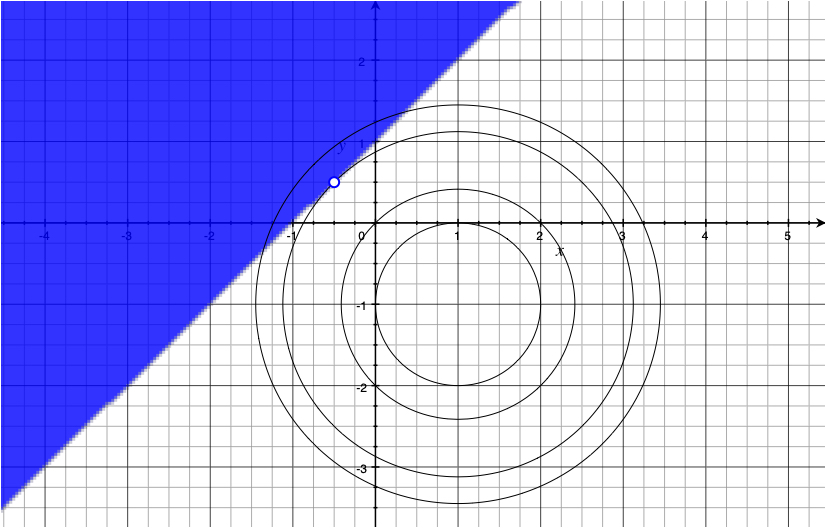
\includegraphics[width=0.8\textwidth]{tujie}
		\caption{\label{fig}图解法图示}
	\end{figure}
	
	使用最优性条件求解,记$f(x)=(x_1-1)^2+(x_2+1)^2,g(x)=-x_1+x_2-1$,计算导数如下:
	\begin{equation}
%	\begin{aligned}
	\bigtriangledown f(x)=\left[
	\begin{array}{c}
	2(x_1-1) \\
	2(x_2+1)
	\end{array}
	\right],\quad\bigtriangledown g(x)=\left[
	\begin{array}{c}
	-1 \\
	1
	\end{array}
	\right]
%	\end{aligned}
	\end{equation}
    最优性条件为:
    \begin{equation}
    \left\{
    \begin{array}{c}
    2(x_1-1)+w=0 \\
    2(x_2+1)-w=0 \\
    w(-x_1+x_2-1)=0 \\
    w \ge 0 \\
    -x_1+x_2-1 \ge 0
    \end{array}
    \right.
    \end{equation}
    解得:$x_1=-0.5,x_2=0.5,w=3$满足条件,代入得到最优值为$\frac{9}{2}$
    \item Lagrange函数为$L(x,w)=f(x)-wg(x)=(x_1-1)^2+(x_2+1)^2-w(-x_1+x_2-1)$
    
    计算对偶问题的目标函数如下:
    
    \begin{equation}
    \begin{aligned}
    \theta(w)&=\inf \{L(x,w)|x\in \mathbb{R}^2\} \\
    &=\inf\{(x_1-1)^2+(x_2+1)^2-w(-x_1+x_2-1)\} \\
    &=\inf\{x_1^2-2x_1+wx_1\}+\inf\{x_2^2+2x_2-wx_2\}+w+2 \\
    &=-\frac{1}{4}(w^2-4w+4)-\frac{1}{4}(w^2-4w+4)+w+2 \\
    &=-\frac{1}{2}w^2+3w
    \end{aligned}
    \end{equation}
    
    因此对偶问题为:
    \begin{equation}
    \begin{aligned}
    \max\quad &-\frac{1}{2}w^2+3w \\
    s.t.\quad &w\ge0
    \end{aligned}
    \end{equation}
\end{enumerate}
\end{proof}
\end{document}